% Figure 1: NutriMATURE construction and evaluation, drawn in TikZ.
% Two additions over the previous raster figure:
%   - a fourth null-control box, D: fitted trend
%   - an "agreement input A -> C" box under "Scores under test"
% Layout uses explicit column anchors and a common top edge, so columns cannot drift into
% one another; every card declares its own text width and no text is clipped.
% Compile: tectonic fig1_protocol.tex   (standalone; the PDF contains the figure only)
\documentclass[border=4pt]{standalone}
\usepackage[T1]{fontenc}
\usepackage{amsmath,amssymb}
\usepackage{tikz}
\usetikzlibrary{positioning,fit,backgrounds,calc,arrows.meta}

\definecolor{cStream}{HTML}{3B6FB6}\definecolor{cAnn}{HTML}{2E8B57}
\definecolor{cUnit}{HTML}{C99700}\definecolor{cScore}{HTML}{5B4EA8}
\definecolor{cProto}{HTML}{B3402F}\definecolor{cNull}{HTML}{2A8C80}
\definecolor{cNew}{HTML}{FFF3D0}\definecolor{bNew}{HTML}{B3402F}
\definecolor{harm}{HTML}{E23B32}\definecolor{prot}{HTML}{2F6FC0}
\definecolor{nul}{HTML}{8A8A8A}\definecolor{unc}{HTML}{C9C9C9}

\begin{document}
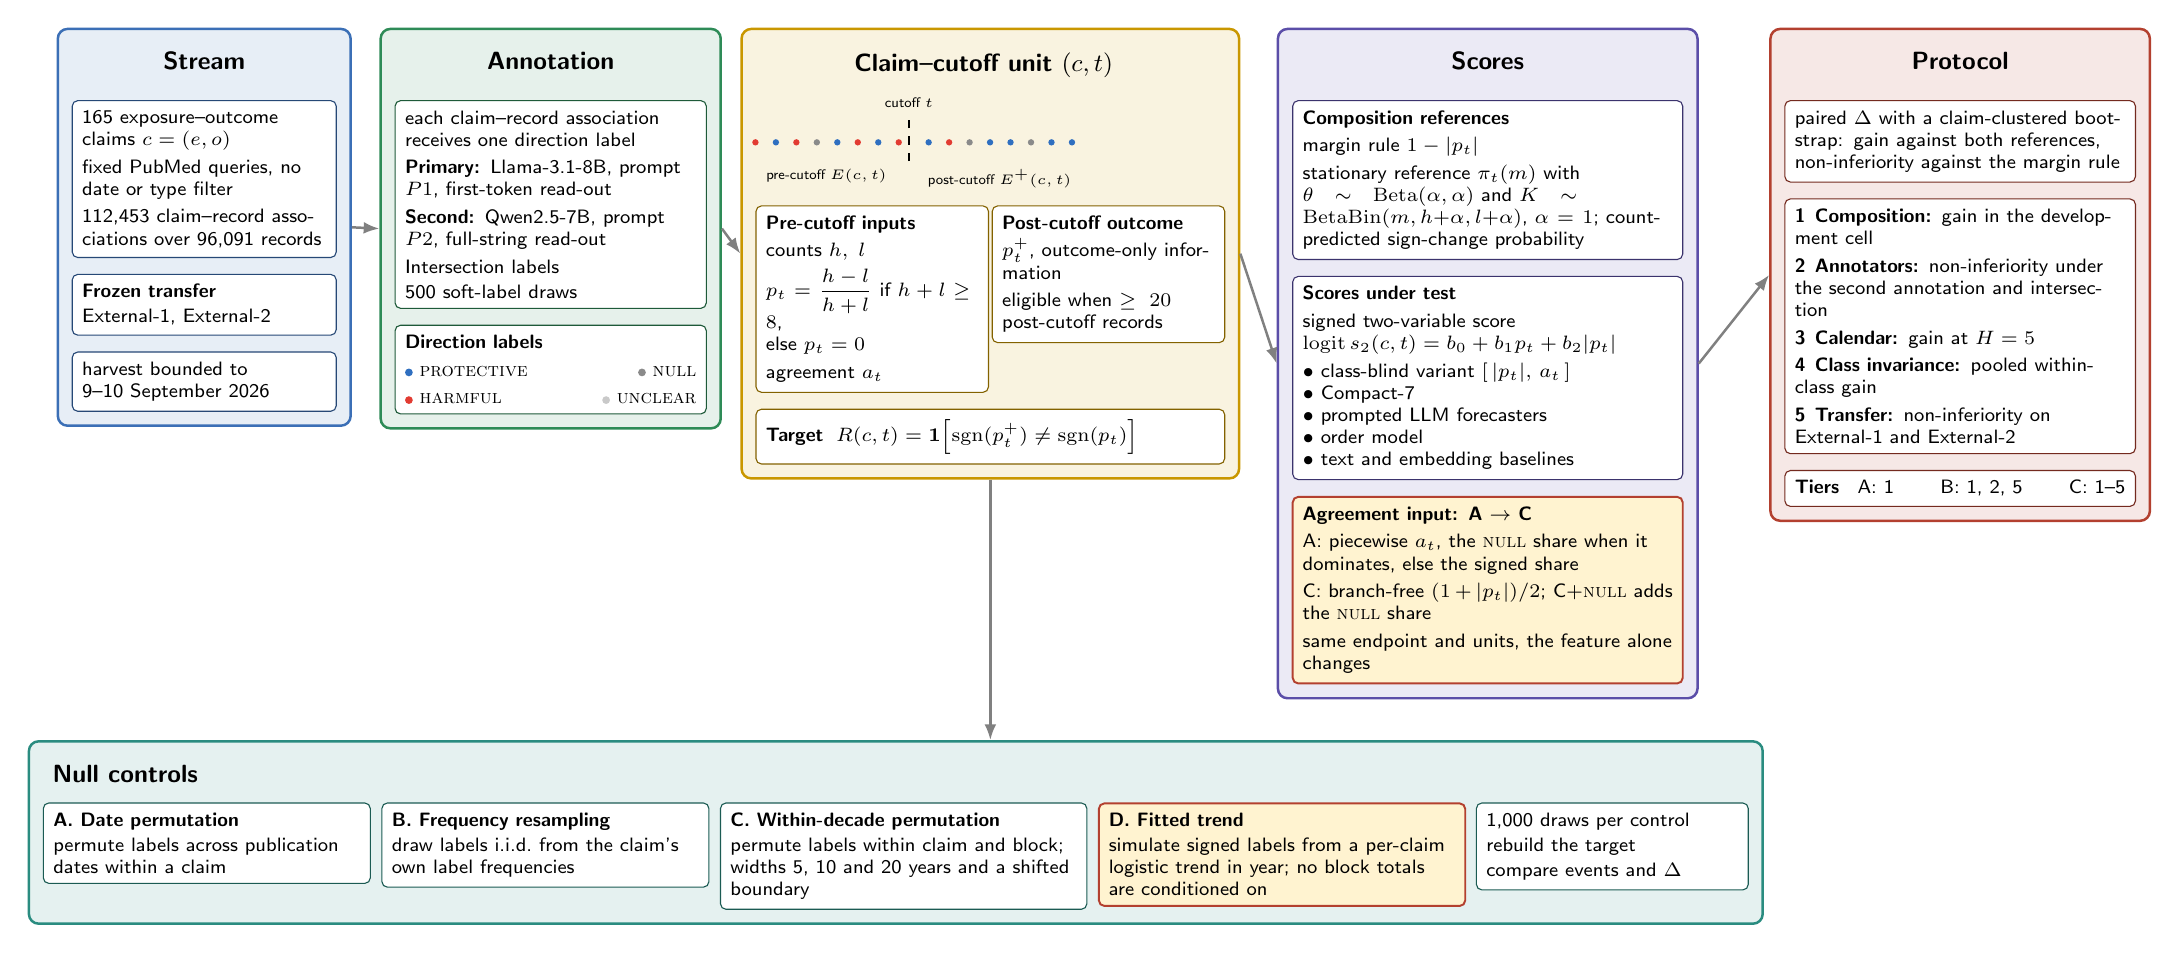
\begin{tikzpicture}[
  font=\sffamily\scriptsize,
  hdr/.style={font=\sffamily\bfseries\small, anchor=north},
  card/.style 2 args={draw=#1!65!black, fill=white, rounded corners=2pt, line width=0.4pt,
                      inner sep=3.6pt, align=left, text width=#2, anchor=north},
  newc/.style={draw=bNew, fill=cNew, rounded corners=2pt, line width=0.7pt,
               inner sep=3.6pt, align=left, anchor=north},
  panel/.style={draw=#1, fill=#1!12, rounded corners=3.5pt, line width=0.9pt, inner sep=5pt},
  arr/.style={-{Latex[length=2mm,width=1.5mm]}, line width=0.9pt, draw=black!50},
]
\def\topy{0}

% ============================================================ 1 STREAM  (x = 0)
\node[hdr] (h1) at (0,\topy) {Stream};
\node[card={cStream}{31mm}] (s1) at ($(h1.south)+(0,-2.6mm)$)
  {165 exposure--outcome claims $c=(e,o)$\\[2pt]
   fixed PubMed queries, no date or type filter\\[2pt]
   112{,}453 claim--record associations over 96{,}091 records};
\node[card={cStream}{31mm}] (s2) at ($(s1.south)+(0,-2mm)$)
  {\textbf{Frozen transfer}\\[1pt] External-1, External-2};
\node[card={cStream}{31mm}] (s3) at ($(s2.south)+(0,-2mm)$)
  {harvest bounded to\\ 9--10 September 2026};
\begin{scope}[on background layer]
  \node[panel=cStream, fit=(h1)(s1)(s2)(s3)] (P1) {};
\end{scope}

% ============================================================ 2 ANNOTATION  (x = 4.4cm)
\node[hdr] (h2) at (4.4,\topy) {Annotation};
\node[card={cAnn}{37mm}] (a1) at ($(h2.south)+(0,-2.6mm)$)
  {each claim--record association receives one direction label\\[2pt]
   \textbf{Primary:} Llama-3.1-8B, prompt $P1$, first-token read-out\\[2pt]
   \textbf{Second:} Qwen2.5-7B, prompt $P2$, full-string read-out\\[2pt]
   Intersection labels\\[1pt] 500 soft-label draws};
\node[card={cAnn}{37mm}] (a2) at ($(a1.south)+(0,-2mm)$)
  {\textbf{Direction labels}\\[2pt]
   \tikz\fill[prot](0,0)circle(1.4pt); \textsc{protective}\hfill
   \tikz\fill[nul](0,0)circle(1.4pt); \textsc{null}\\[2pt]
   \tikz\fill[harm](0,0)circle(1.4pt); \textsc{harmful}\hfill
   \tikz\fill[unc](0,0)circle(1.4pt); \textsc{unclear}};
\begin{scope}[on background layer]
  \node[panel=cAnn, fit=(h2)(a1)(a2)] (P2) {};
\end{scope}

% ============================================================ 3 CLAIM-CUTOFF UNIT  (x = 9.9cm)
\node[hdr] (h3) at (9.9,\topy) {Claim--cutoff unit $(c,t)$};
% timeline, drawn from an explicit left edge so the dots cannot drift
\coordinate (T0) at ($(h3.south)+(-29mm,-7mm)$);
\foreach \i/\c in {0/harm,1/prot,2/harm,3/nul,4/prot,5/harm,6/prot,7/harm}
  {\fill[\c] ($(T0)+(\i*2.6mm,0)$) circle (1.15pt);}
\draw[dashed,line width=0.5pt] ($(T0)+(19.5mm,-2.4mm)$) -- ($(T0)+(19.5mm,3.4mm)$);
\node[font=\sffamily\tiny,anchor=south] at ($(T0)+(19.5mm,3.2mm)$) {cutoff $t$};
\foreach \i/\c in {0/prot,1/harm,2/nul,3/prot,4/prot,5/nul,6/prot,7/prot}
  {\fill[\c] ($(T0)+(22mm+\i*2.6mm,0)$) circle (1.15pt);}
\node[font=\sffamily\tiny,anchor=north] at ($(T0)+(9mm,-2.2mm)$) {pre-cutoff $E(c,t)$};
\node[font=\sffamily\tiny,anchor=north] at ($(T0)+(31mm,-2.2mm)$) {post-cutoff $E^{+}(c,t)$};
\coordinate (U0) at ($(T0)+(0,-8mm)$);
\node[card={cUnit}{27mm}, anchor=north west] (u1) at (U0)
  {\textbf{Pre-cutoff inputs}\\[2pt]
   counts $h,\;l$\\[2pt]
   $p_t=\dfrac{h-l}{h+l}$ if $h+l\ge 8$,\\ else $p_t=0$\\[2pt]
   agreement $a_t$};
\node[card={cUnit}{27mm}, anchor=north west] (u2) at ($(U0)+(30mm,0)$)
  {\textbf{Post-cutoff outcome}\\[2pt]
   $p_t^{+}$, outcome-only information\\[2pt]
   eligible when $\ge 20$ post-cutoff records};
\node[card={cUnit}{57mm}, anchor=north west] (u3) at ($(u1.south west)+(0,-2mm)$)
  {\textbf{Target}\; $R(c,t)=\mathbf{1}\!\left[\operatorname{sgn}(p_t^{+})\neq\operatorname{sgn}(p_t)\right]$};
\begin{scope}[on background layer]
  \node[panel=cUnit, fit=(h3)(T0)(u1)(u2)(u3)] (P3) {};
\end{scope}

% ============================================================ 4 SCORES  (x = 16.3cm)
\node[hdr] (h4) at (16.3,\topy) {Scores};
\node[card={cScore}{47mm}] (c1) at ($(h4.south)+(0,-2.6mm)$)
  {\textbf{Composition references}\\[2pt]
   margin rule $1-|p_t|$\\[2pt]
   stationary reference $\pi_t(m)$ with
   $\theta\sim\mathrm{Beta}(\alpha,\alpha)$ and
   $K\sim\mathrm{BetaBin}(m,h{+}\alpha,l{+}\alpha)$, $\alpha=1$;
   count-predicted sign-change probability};
\node[card={cScore}{47mm}] (c2) at ($(c1.south)+(0,-2mm)$)
  {\textbf{Scores under test}\\[2pt]
   signed two-variable score\\
   $\operatorname{logit}s_2(c,t)=b_0+b_1p_t+b_2|p_t|$\\[2pt]
   $\bullet$ class-blind variant $[\,|p_t|,\,a_t\,]$\\
   $\bullet$ Compact-7\\
   $\bullet$ prompted LLM forecasters\\
   $\bullet$ order model\\
   $\bullet$ text and embedding baselines};
\node[newc, text width=47mm] (c3) at ($(c2.south)+(0,-2mm)$)
  {\textbf{Agreement input: A $\rightarrow$ C}\\[2pt]
   A: piecewise $a_t$, the \textsc{null} share when it dominates, else the signed share\\[2pt]
   C: branch-free $(1+|p_t|)/2$; C$+$\textsc{null} adds the \textsc{null} share\\[2pt]
   same endpoint and units, the feature alone changes};
\begin{scope}[on background layer]
  \node[panel=cScore, fit=(h4)(c1)(c2)(c3)] (P4) {};
\end{scope}

% ============================================================ 5 PROTOCOL  (x = 22.3cm)
\node[hdr] (h5) at (22.3,\topy) {Protocol};
\node[card={cProto}{42mm}] (p0) at ($(h5.south)+(0,-2.6mm)$)
  {paired $\Delta$ with a claim-clustered bootstrap: gain against both references,
   non-inferiority against the margin rule};
\node[card={cProto}{42mm}] (p1) at ($(p0.south)+(0,-2mm)$)
  {\textbf{1\;\,Composition:} gain in the development cell\\[2pt]
   \textbf{2\;\,Annotators:} non-inferiority under the second annotation and intersection\\[2pt]
   \textbf{3\;\,Calendar:} gain at $H=5$\\[2pt]
   \textbf{4\;\,Class invariance:} pooled within-class gain\\[2pt]
   \textbf{5\;\,Transfer:} non-inferiority on External-1 and External-2};
\node[card={cProto}{42mm}] (p2) at ($(p1.south)+(0,-2mm)$)
  {\textbf{Tiers}\;\; A: 1\hfill B: 1, 2, 5\hfill C: 1--5};
\begin{scope}[on background layer]
  \node[panel=cProto, fit=(h5)(p0)(p1)(p2)] (P5) {};
\end{scope}

% ============================================================ stage arrows
\foreach \a/\b in {P1/P2,P2/P3,P3/P4,P4/P5}{\draw[arr] (\a.east) -- (\b.west);}

% ============================================================ NULL CONTROLS band
% anchored below the LOWEST of the five columns, not below the first one, so a tall
% column can never overlap the band
\begin{scope}[on background layer]
  \node[fit=(P1)(P2)(P3)(P4)(P5), inner sep=0pt, draw=none, fill=none] (TOPROW) {};
\end{scope}
\coordinate (NB) at ($(P1.west|-TOPROW.south)+(-5pt,-7mm)$);
\node[hdr, anchor=north west] (h6) at (NB) {Null controls};
\coordinate (N0) at ($(NB)+(0,-6mm)$);
\node[card={cNull}{39mm}, anchor=north west] (n1) at (N0)
  {\textbf{A. Date permutation}\\[1pt] permute labels across publication dates within a claim};
\node[card={cNull}{39mm}, anchor=north west] (n2) at ($(N0)+(43mm,0)$)
  {\textbf{B. Frequency resampling}\\[1pt] draw labels i.i.d.\ from the claim's own label frequencies};
\node[card={cNull}{44mm}, anchor=north west] (n3) at ($(N0)+(86mm,0)$)
  {\textbf{C. Within-decade permutation}\\[1pt] permute labels within claim and block; widths 5, 10 and 20 years and a shifted boundary};
\node[newc, text width=44mm, anchor=north west] (n4) at ($(N0)+(134mm,0)$)
  {\textbf{D. Fitted trend}\\[1pt] simulate signed labels from a per-claim logistic trend in year; no block totals are conditioned on};
\node[card={cNull}{32mm}, anchor=north west] (n5) at ($(N0)+(182mm,0)$)
  {1{,}000 draws per control\\[1pt] rebuild the target\\[1pt] compare events and $\Delta$};
\begin{scope}[on background layer]
  \node[panel=cNull, fit=(h6)(n1)(n2)(n3)(n4)(n5)] (P6) {};
\end{scope}
\draw[arr] (P3.south) -- (P3.south|-P6.north);

\end{tikzpicture}
\end{document}
